% Copyright (c) 2015 Daniele Masini - d.masini.it@gmail.com
% Copyright (c) 2016 Daniele Zambelli - daniele.zambelli@gmail.com

\section{Esercizi}

\subsection{Esercizi riepilogativi}

\begin{esercizio}
\label{ese:4.1}
Quali tra le seguenti sono proprietà del parallelogrammo?
\begin{enumeratea}
\item Ciascuna diagonale lo divide in due triangoli 
uguali\hfill\boxV\quad\boxF
\item Gli angoli opposti sono uguali\hfill\boxV\quad\boxF
\item Tutti i lati sono uguali\hfill\boxV\quad\boxF
\item Gli angoli sulla base sono uguali\hfill\boxV\quad\boxF
\item Le diagonali sono perpendicolari\hfill\boxV\quad\boxF
\item Gli angoli sono tutti congruenti\hfill\boxV\quad\boxF
\item Le diagonali sono anche bisettrici\hfill\boxV\quad\boxF
\end{enumeratea}
\end{esercizio}

\begin{esercizio}
\label{ese:4.2}
Vero o Falso?
\begin{enumeratea}
\item Un quadrilatero che ha i lati consecutivi a due a due 
congruenti è un deltoide\hfill\boxV\quad\boxF
\item Un quadrilatero che ha una sola coppia di lati opposti uguali è 
un trapezio\hfill\boxV\quad\boxF
\item Il trapezio scaleno ha tutti i lati diversi tra di loro per 
lunghezza\hfill\boxV\quad\boxF
\item Gli angoli adiacenti alla base maggiore di un trapezio 
rettangolo sono uno retto e uno acuto\hfill\boxV\quad\boxF
\item Un trapezio scaleno può avere due angoli opposti 
ottusi\hfill\boxV\quad\boxF
\item In un trapezio isoscele gli angoli adiacenti alla base minore 
sono ottusi\hfill\boxV\quad\boxF
\item In un trapezio isoscele sono congruenti le proiezioni dei lati 
obliqui sulla base maggiore\tab\hfill\boxV\quad\boxF
\item Le diagonali di un deltoide si incontrano nel loro punto medio 
comune\hfill\boxV\quad\boxF
\item Nel parallelogramma gli angoli adiacenti allo stesso lato sono 
supplementari\hfill\boxV\quad\boxF
\item Nel parallelogramma una delle due diagonali lo divide in due 
triangoli isosceli\tab\tab\tab\hfill\boxV\quad\boxF
\item Se le diagonali di un quadrilatero si dividono a metà allora è 
un parallelogramma\tab\tab\hfill\boxV\quad\boxF
\item Le diagonali del rombo sono anche 
bisettrici\hfill\boxV\quad\boxF
\item Se le diagonali di un parallelogramma sono uguali il 
parallelogramma è un quadrato\tab\tab\hfill\boxV\quad\boxF
\item Un parallelogramma che ha un angolo retto è un 
rettangolo\hfill\boxV\quad\boxF
\item Un parallelogramma che ha due lati consecutivi congruenti è un 
quadrato\hfill\boxV\quad\boxF
\item Un quadrilatero con due lati opposti congruenti è un 
trapezio\hfill\boxV\quad\boxF
\item Il rombo è anche un rettangolo\hfill\boxV\quad\boxF
\item Il rombo è anche quadrato\hfill\boxV\quad\boxF
\item Il rettangolo è anche parallelogrammo\hfill\boxV\quad\boxF
\item Il quadrato è anche rombo\hfill\boxV\quad\boxF
\item Il trapezio è anche parallelogrammo\hfill\boxV\quad\boxF
\item Alcuni rettangoli sono anche rombi\hfill\boxV\quad\boxF
\end{enumeratea}
\end{esercizio}

\begin{multicols}{2}

\subsubsection*{Dimostra le seguenti proprietà}

\begin{esercizio}
\label{ese:4.3}
Due parallelogrammi sono congruenti se hanno congruenti due lati 
consecutivi e l'angolo compreso.
\end{esercizio}

\begin{esercizio}
\label{ese:4.4}
Due rettangoli sono congruenti se hanno congruenti due lati 
consecutivi.
\end{esercizio}

\begin{esercizio}
\label{ese:4.5}
Due rombi sono congruenti se hanno congruenti le due diagonali.
\end{esercizio}

\begin{esercizio}
\label{ese:4.6}
Le diagonali di un trapezio isoscele si dividono in parti 
rispettivamente congruenti.
\end{esercizio}

\begin{esercizio}
\label{ese:4.7}
In un trapezio isoscele, la retta che congiunge i punti medi delle 
basi è perpendicolare alle basi stesse, ed interseca le rette dei 
lati obliqui nel loro punto d’intersezione.
\end{esercizio}

\begin{esercizio}
\label{ese:4.8}
Se un trapezio ha tre lati congruenti, le diagonali sono bisettrici 
degli angoli adiacenti alla base maggiore.
\end{esercizio}

\begin{esercizio}
\label{ese:4.9}
Dimostra che un rombo è diviso da una sua diagonale in due triangoli 
isosceli congruenti.
\end{esercizio}

\begin{esercizio}
\label{ese:4.10}
In un triangolo $ABC$ prolunga la mediana $AM$ di un segmento $MD$ 
congruente ad $AM$. Dimostra che il quadrilatero $ABCD$ è un 
parallelogramma.
\end{esercizio}

\begin{esercizio}
\label{ese:4.11}
Sia $ABCD$ un parallelogramma, siano $M$, $N$, $O$ e $P$ i punti medi 
dei lati. Dimostra che $MNOP$ è un parallelogramma.
\end{esercizio}

\begin{esercizio}
\label{ese:4.12}
Nel parallelogramma $ABCD$ prolunga di segmenti congruenti ciascun 
lato e sempre nello stesso senso. Dimostra che i nuovi vertici che si 
ottengono formano un parallelogramma.
\end{esercizio}

\begin{esercizio}
\label{ese:4.13}
Nel parallelogramma $ABCD$ si prendono sui lati opposti $AB$ e $CD$ i 
punti $E$ ed $F$ tali che $AE$ sia congruente a $CF$. Dimostra che 
anche $AECF$ è un parallelogramma.
\end{esercizio}

\begin{esercizio}
\label{ese:4.14}
Di un triangolo $ABC$ prolunga i lati $AB$ e $CB$ rispettivamente di 
due segmenti $BD$ e $BE$ tali che $AB\cong BD$ e $CB\cong BE$. 
Dimostra che $ACDE$ è un parallelogramma.
\end{esercizio}

\begin{esercizio}
\label{ese:4.15}
Unendo i punti medi di due lati opposti di un parallelogramma si 
ottengono due parallelogrammi.
\end{esercizio}

\begin{esercizio}
\label{ese:4.16}
Sulle diagonali $AC$ e $BD$ di un parallelogramma prendi i punti $A'$ 
e $C'$ su $AC$ in modo che $AA'\cong CC'$ su $BD$ prendi i punti $B'$ 
e $D'$ in modo che $BB'\cong DD'$. Dimostra che $A'B'C'D'$ è un 
parallelogramma.
\end{esercizio}

\begin{esercizio}
\label{ese:4.17}
Dato un parallelogramma $ABCD$ prolunga il lati nel seguente modo: 
$CD$ di un segmento $DE$, $DA$ di un segmento $DF$, $AB$ di un 
segmento $BG$, $BC$ di un segmento $CH$. Dimostra che se $DE\cong 
AF\cong BG\cong CH$ allora $EFGH$ è anche un parallelogramma.
\end{esercizio}

\begin{esercizio}
\label{ese:4.18}
Dato un segmento $AB$, sia $M$ il suo punto medio. Traccia 
rispettivamente da $A$ e da $B$ le rette $r$ ed $s$ parallele tra 
loro. Dal punto $M$ traccia una trasversale $t$ alle due rette che 
incontra $r$ in $C$ ed $s$ in $D$. Dimostra che $CADB$ è un 
parallelogramma.
\end{esercizio}

\begin{esercizio}
\label{ese:4.19}
Dimostra che in un parallelogramma $ABCD$ i due vertici opposti $A$ e 
$C$ sono equidistanti dalla diagonale $BD$.
\end{esercizio}

\begin{esercizio}
\label{ese:4.20}
Prolunga la mediana $AM$ di un triangolo isoscele di vertice $A$ di 
un segmento $MD$ congruente ad $AM$. Dimostra che $ABCD$ è un rombo.
\end{esercizio}

\begin{esercizio}
\label{ese:4.21}
Nel parallelogramma $ABCD$ sia $M$ il punto medio di $AB$ ed $N$ il 
punto medio di $DC$. Sia $P$ il punto di intersezione di $AN$ con 
$DM$ e $Q$ il punto di intersezione di $CM$ con $BN$. Dimostra che 
$PNAM$ è un rombo.
\end{esercizio}

\begin{esercizio}
\label{ese:4.22}
Dimostra che se un rombo ha le diagonali congruenti allora è un 
quadrato.
\end{esercizio}

\begin{esercizio}
\label{ese:4.23}
Dimostra che congiungendo i punti medi dei lati di un rettangolo si 
ottiene un rombo.
\end{esercizio}

\begin{esercizio}
\label{ese:4.24}
Dato un parallelogramma $ABCD$, siano $H$ e $K$ due punti della 
diagonale $AC$ in modo che $DH$ e $BK$ siano perpendicolari ad $AC$. 
Dimostra che $AH\cong KC$.
\end{esercizio}

\begin{esercizio}
\label{ese:4.25}
Sia $ABCD$ un trapezio di basi $BC$ e $AD$. Sia $r$ la bisettrice 
dell'angolo in $A$ ed $s$ la bisettrice dell'angolo in $B$. Dimostra 
che $r$ ed $s$ sono perpendicolari.
\end{esercizio}

\begin{esercizio}
\label{ese:4.26}
Nel parallelogramma $ABCD$ prolunga il lato $AB$ del segmento $AE$ e 
il lato $DC$ del segmento $CF$ congruente ad $AE$. Dimostra che anche 
$EBFD$ è un parallelogramma.
\end{esercizio}

\begin{esercizio}
\label{ese:4.27}
In un trapezio $ABCD$ la diagonale $AC$ è congruente alla base 
maggiore $AB$. Sia $M$ il punto medio del lato obliquo $BC$. Prolunga 
$AM$ di un segmento $ME$ congruente ad $AM$. Dimostra che $ABEC$ è un 
rombo.
\end{esercizio}

\begin{esercizio}
\label{ese:4.28}
Nel trapezio isoscele $ABCD$ con la base maggiore doppia della base 
minore, unisci il punto medio $M$ di $AB$ con gli estremi della base 
$DC$. Dimostra che $AMCD$ è un parallelogramma.
\end{esercizio}

\begin{esercizio}
\label{ese:4.29}
Nel trapezio isoscele $ABCD$ i punti $M$ e $N$ sono rispettivamente i 
punti medi delle basi $AB$ e $DC$. Dimostra che $MNCB$ è un trapezio 
rettangolo.
\end{esercizio}

\begin{esercizio}
\label{ese:4.30}
Siano $M$ e $N$ i punti medi dei lati obliqui di un trapezio isoscele 
$ABCD$. Dimostra che $BCMN$ è un trapezio isoscele.
\end{esercizio}

\begin{esercizio}
\label{ese:4.31}
Nel triangolo isoscele $ABC$ siano $BH$ e $BK$ le perpendicolari ai 
lati obliqui $AC$ e $AB$. Dimostra che $BCHK$ è un trapezio isoscele.
\end{esercizio}

\begin{esercizio}
\label{ese:4.32}
Dimostra che le proiezioni dei lati obliqui di un trapezio isoscele 
sulla base maggiore sono congruenti.
\end{esercizio}

\begin{esercizio}
\label{ese:4.33}
Nel triangolo isoscele $ABC$, di base $BC$, traccia le bisettrici 
agli angoli adiacenti alla base. Detti $D$ ed $E$ i punti di incontro 
di dette bisettrici rispettivamente con $AC$ e $AB$, dimostra che 
$EBCD$ è un trapezio isoscele.
\end{esercizio}

\begin{esercizio}
\label{ese:4.34}
Dimostra che in un trapezio isoscele che ha la base maggiore doppia 
della minore, le diagonali sono anche bisettrici degli angoli 
adiacenti alla base maggiore.
\end{esercizio}

\begin{esercizio}
\label{ese:4.35}
In un trapezio, il segmento che unisce i punti medi dei lati obliqui 
è parallelo alle basi e congruente alla loro semisomma.
\end{esercizio}

\begin{esercizio}
\label{ese:4.36}
Dato un qualsiasi quadrilatero $ABCD$, il quadrilatero non 
intrecciato avente come vertici i punti medi dei lati di $ABCD$ è un 
parallelogramma.
\end{esercizio}

\begin{esercizio}
\label{ese:4.37}
Il quadrilatero avente come vertici i punti medi dei lati di un 
trapezio isoscele è un rombo.
\end{esercizio}

\begin{esercizio}
\label{ese:4.38}
Dimostrare che, in un trapezio, il segmento che congiunge i punti 
medi dei lati non paralleli è uguale alla semisomma delle basi.
\end{esercizio}

\begin{esercizio}
\label{ese:4.39}
Dato un parallelogramma $ABCD$, si consideri il punto medio $M$ del 
lato $AB$, si congiunga il vertice $D$ con il punto $M$, si congiunga 
il vertice $A$ con il punto medio $N$ del segmento $DM$. Dimostrare 
che la retta $AN$ divide la diagonale $DB$ del parallelogramma in due 
parti di cui una è il doppio dell'altra.
\end{esercizio}

\begin{esercizio}
\label{ese:4.40}
Dato un triangolo qualunque $ABC$, si consideri il punto medio $M$ 
del lato $AB$, si consideri il segmento parallelo al lato $BC$ che 
parte da $M$ ed incontra il lato $AC$ nel punto $N$, si prolunghi 
questo segmento di un segmento $ND$ uguale ad $MN$. Dimostrare che il 
quadrilatero $MDCB$ è un parallelogramma.
\end{esercizio}

\begin{esercizio}
\label{ese:4.41}
Dato un quadrato $ABCD$ di centro $O$, siano $H$ e $K$ due punti 
sulla diagonale $AC$ simmetrici rispetto ad $O$. Dimostra che il 
quadrilatero $BHDK$ è un rombo. 
\end{esercizio}

\begin{esercizio}
\label{ese:4.42}
Dimostrare che un trapezio è isoscele se il punto medio della sua 
base maggiore è equidistante dagli estremi della base minore.
\end{esercizio}

\begin{esercizio}
\label{ese:4.43}
In un trapezio isoscele $ABCD$ (con base maggiore $AB$ e lati obliqui 
congruenti $BC$ e $AD$) sia $M$ il punto medio della base maggiore; 
prolungare $MC$ e $MD$ rispettivamente dei segmenti $CE$ e $DF$ fra 
loro congruenti. Dimostrare che il quadrilatero $ABEF$ è un trapezio 
isoscele.
\end{esercizio}

\begin{esercizio}
\label{ese:4.44}
Nel parallelogramma $ABCD$ si traccino da $A$ e da $C$ le 
perpendicolari alla diagonale $BD$; siano rispettivamente $E$ ed $F$ 
i punti di intersezione delle perpendicolari con la diagonale. 
Dimostra che $DE$ è congruente a $FB$ e che $AFCE$ è un 
parallelogramma.
\end{esercizio}

\begin{esercizio}
\label{ese:4.45}
Dato un parallelogramma $ABCD$, si consideri il punto medio $M$ del 
lato $AB$, si congiunga il vertice $D$ con il punto $M$, si congiunga 
il vertice $A$ con il punto medio $N$ del segmento $DM$. Dimostrare 
che la retta $AN$ divide la diagonale $DB$ del parallelogramma in due 
parti di cui una è il doppio dell'altra.	
\end{esercizio}

\begin{esercizio}
\label{ese:4.46}
Dato un triangolo qualunque $ABC$, si consideri il punto medio $M$ 
del lato $AB$, si consideri il segmento parallelo al lato $BC$ che 
parte da $M$ ed incontra il lato $AC$ nel punto $N$, si prolunghi 
questo segmento di un segmento $ND$ uguale ad $MN$. Dimostrare che il 
quadrilatero $MDCB$ è un parallelogramma.
\end{esercizio}

\begin{esercizio}
\label{ese:4.47}
Dato un quadrato $ABCD$ di centro $O$, siano $H$ e $K$ due punti 
sulla diagonale $AC$ simmetrici rispetto ad $O$. Dimostra che il 
quadrilatero $BHDK$ è un rombo.
\end{esercizio}

\begin{esercizio}
\label{ese:4.48}
Le diagonali di un trapezio isoscele dividono il trapezio in quattro 
triangoli, dei quali due triangoli sono isosceli e aventi gli angoli 
ordinatamente congruenti, mentre gli altri due triangoli sono 
congruenti.
\end{esercizio}

\begin{esercizio}
\label{ese:4.49}
Dimostra che il quadrilatero che si ottiene congiungendo i punti medi 
dei lati di un quadrilatero qualunque è un parallelogramma.
\end{esercizio}

\begin{esercizio}
\label{ese:4.50}
Che tipo di quadrilatero si ottiene congiungendo i punti medi dei 
lati di un rombo?
\end{esercizio}

\begin{esercizio}
\label{ese:4.51}
Che tipo di quadrilatero si ottiene congiungendo i punti medi dei 
lati di un rettangolo?
\end{esercizio}

\begin{esercizio}
\label{ese:4.52}
Dimostra che in un parallelogramma due vertici opposti sono 
equidistanti dalla diagonale avente per estremi gli altri due vertici.
\end{esercizio}

\begin{esercizio}
\label{ese:4.53}
In un parallelogramma $ABCD$ sia $M$ il punto medio di $AB$ e $N$ il 
punto medio di $DC$. Dimostra che $DMBN$ è un parallelogramma.
\end{esercizio}

\begin{esercizio}
\label{ese:4.54}
Dimostra che se in un parallelogramma le bisettrici di due angoli 
consecutivi si incontrano in un punto del lato opposto allora il 
parallelogramma ha un lato che è il doppio dell'altro.
\end{esercizio}

\begin{esercizio}
\label{ese:4.55}
Nel trapezio isoscele $ABCD$ le bisettrici degli angoli alla base 
maggiore $DC$ si incontrano in un punto $E$ sulla base minore. 
Dimostrare che $E$ è il punto medio della base minore.
\end{esercizio}

\begin{esercizio}
\label{ese:4.56}
Dimostra che un parallelogramma che ha tutte le altezze congruenti è 
un rombo.
\end{esercizio}

\begin{esercizio}
\label{ese:4.57}
In un trapezio le bisettrici degli angoli adiacenti alla base minore 
si intersecano in un punto della base maggiore. Dimostra che la base 
maggiore è congruente alla somma dei lati obliqui.
\end{esercizio}

\begin{esercizio}
\label{ese:4.58}
Disegna un trapezio isoscele con le diagonali perpendicolari. 
Dimostrare che il quadrilatero formato dai punti medi dei lati del 
trapezio è un quadrato.
\end{esercizio}

\begin{esercizio}
\label{ese:4.59}
Sia $AD$ bisettrice del triangolo $ABC$. Da $D$ traccia le parallele 
ai lati $AB$ e $AC$, detto $E$ il punto di intersezione del lato $AC$ 
con la parallela ad $AB$ ed $F$ il punto di intersezione del lato 
$AB$ con la parallela ad $AC$, dimostra che $AEDF$ è un rombo.
\end{esercizio}

\end{multicols}

\noindent\begin{minipage}{0.6\textwidth}\parindent15pt
\begin{esercizio}[Prove invalsi 2003]
\label{ese:4.60}
Il quadrilatero nella figura a fianco è simmetrico rispetto alla 
retta $AC$.
Sapendo che $B\widehat{A}C = 30\grado$ e $C\widehat{D}A = 70\grado$, 
quanto vale $B\widehat{C}D$?
\begin{enumeratea}
\item $140\grado$;
\item $150\grado$;
\item $160\grado$;
\item $165\grado$;
\item Le informazioni sono insufficienti.
\end{enumeratea}
\end{esercizio}
\end{minipage}\hfil
\begin{minipage}{0.4\textwidth}
	\centering% Copyright (c) 2015 Daniele Masini - d.masini.it@gmail.com

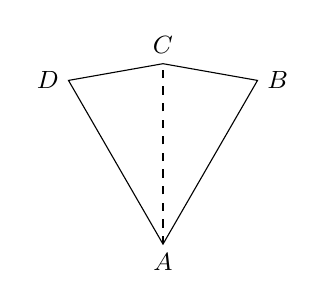
\begin{tikzpicture}[scale=1.2,font=\small]
\usetikzlibrary{calc, through, intersections}

\begin{scope}
\coordinate (a) at (0,0);
\coordinate (b) at (60:2);
\coordinate (d) at (120:2);
\coordinate (m) at ($(a)!.5!(b)$);

\path (b) -- +(170:1) coordinate (r2);
\coordinate (s2) at (90:1);
\coordinate (c) at (intersection of b--r2 and a--s2);
\draw[dashed] (a) -- (c);

\draw (a) node[below] {$A$} -- (b) node[right] {$B$} -- (c) node[above] {$C$} -- (d) node[left] {$D$} -- cycle;

\end{scope}

\end{tikzpicture}

\end{minipage}

\begin{esercizio}[Prove invalsi 2003]
\label{ese:4.61}
Quale fra le seguenti proprietà è falsa per tutti i parallelogrammi?
\begin{enumeratea}
\item I lati opposti sono uguali.
\item Gli angoli adiacenti sono supplementari.
\item Gli angoli opposti sono supplementari.
\item I lati opposti sono paralleli.
\item Le diagonali si dimezzano scambievolmente.
\end{enumeratea}
\end{esercizio}

\begin{esercizio}[Prove invalsi 2004]
\label{ese:4.62}
Quale tra le seguenti affermazioni riferite ad un parallelogramma 
qualsiasi è FALSA?
\begin{enumeratea}
\item I lati opposti sono paralleli.
\item Le diagonali sono uguali.
\item Gli angoli opposti sono uguali.
\item Ogni diagonale divide il parallelogramma in due triangoli 
uguali.
\end{enumeratea}
\end{esercizio}

\begin{esercizio}[Prove invalsi 2005]
\label{ese:4.63}
Quale tra le seguenti affermazioni relative ad un rombo è FALSA?
\begin{multicols}{2}
\begin{enumeratea}
\item Non ha i lati opposti paralleli.
\item Ha tutti i lati uguali.
\item Ha gli angoli opposti uguali.
\item Ha le diagonali perpendicolari.
\end{enumeratea}
\end{multicols}
\end{esercizio}

\begin{esercizio}[Prove invalsi 2005]
\label{ese:4.64}
Quale fra le seguenti condizioni è sufficiente affinché un 
quadrilatero sia un rettangolo?
\begin{enumeratea}
\item I lati opposti siano uguali e un angolo sia retto.
\item Le diagonali si dividano a metà.
\item I lati opposti siano paralleli.
\item Le diagonali siano uguali e un angolo sia retto.
\end{enumeratea}
\end{esercizio}

\begin{esercizio}[Prove invalsi 2006]
\label{ese:4.65}
Quale fra le seguenti affermazioni è vera?
Il quadrilatero avente i vertici nei punti medi dei lati di \ldots{}
\begin{enumeratea}
\item \ldots{} un rettangolo qualsiasi è sempre un quadrato.
\item \ldots{} un trapezio isoscele qualsiasi è un rettangolo.
\item \ldots{} un quadrilatero qualsiasi è un parallelogramma.
\item \ldots{} un quadrato è un rombo, ma non un quadrato.
\end{enumeratea}
\end{esercizio}

\begin{esercizio}[Prove invalsi 2007]
\label{ese:4.66}
Quale fra le seguenti affermazioni è falsa?
\begin{enumeratea}
\item Ogni rettangolo è anche un rombo.
\item Ogni rettangolo è anche un parallelogramma.
\item Ogni quadrato è anche un rombo.
\item Ogni rettangolo ha le diagonali uguali.
\end{enumeratea}
\end{esercizio}

\begin{esercizio}[Prove invalsi 2007]
\label{ese:4.67}
\`E dato un quadrilatero con le diagonali perpendicolari che si 
dimezzano scambievolmente.\\
Alberto afferma: <<Di sicuro si tratta di un quadrato.>>\\
Barbara afferma: <<Non è detto che sia un quadrato, ma di sicuro è un 
rombo.>>\\
Carla afferma: <<Non è detto che sia un quadrato, ma di sicuro è un 
rettangolo.>>\\
Daniele afferma: <<Si tratta certamente di un quadrilatero a forma di 
aquilone.>>\\
Chi ha ragione?
\begin{multicols}{4}
\begin{enumeratea}
\item Alberto;
\item Barbara;
\item Carla;
\item Daniele.
\end{enumeratea}
\end{multicols}
\end{esercizio}


\subsection{Risposte}

\begingroup
\hypersetup{linkcolor=black}

\paragraph{\ref{ese:4.1}.}
a)~V,\quad b)~V,\quad c)~F,\quad d)~F,\quad e)~F,\quad f)~F,\quad 
g)~F.

\paragraph{\ref{ese:4.2}.}
a)~F,\quad b)~F,\quad c)~V,\quad d)~V,\quad e)~F,\quad f)~V,\quad 
g)~V,\quad h)~F,\quad i)~V,\quad j)~F,\quad k)~F,\quad l)~V,\quad 
m)~F,\quad n)~V,\quad o)~V,\quad p)~F,\quad q)~F,\quad r)~F,\quad 
s)~V,\quad t)~V,\quad u)~F,\quad v)~V.

\paragraph{\ref{ese:4.60}.}
c.

\paragraph{\ref{ese:4.61}.}
c.

\paragraph{\ref{ese:4.62}.}
c.

\paragraph{\ref{ese:4.63}.}
a.

\paragraph{\ref{ese:4.64}.}
a.

\paragraph{\ref{ese:4.65}.}
c.

\paragraph{\ref{ese:4.66}.}
a.

\paragraph{\ref{ese:4.67}.}
b.

\endgroup
